% Provenance (never printed): see sources/outline_sources.md (Year 1: insolation with
% latitude and season, the radiative surplus and deficit, meridional heat transport by
% the atmosphere and the ocean, latent heat). Exercise and problem values in the Book 3
% scratch calculator calc/ch27.py; figures from figdata/bachelor-1/insolation.py (Kepler
% orbit of _solar.py) and energy_balance.py (NCEP-NCAR Reanalysis 1, long-term means
% 1991-2020, datasets bachelor-1-ncep-*).
% Physics owns the inverse-square law, the black body and the Stefan-Boltzmann law, the
% seasons and latent heat (recalled). Book 2 (g10) gave the quarter of the solar constant,
% the global budget diagram and its closure, latent and sensible heat in words, the
% annual-mean insolation curve and the poleward transport in words: re-founded here with
% derivations and data. Ch. 1 gave the instantaneous insolation, the declination and the
% rising and setting of the Sun.
\chapter{Straling en warmtetransport}\label{ch:b1:radiation-heat-transport}

Vanaf anderhalf miljoen kilometer afstand is de zonverlichte kant van de aarde een schijf van blauwe zee, bruin land en wit wolkendek. Het zonlicht valt het meest recht op het midden van de schijf, nabij de tropen, en raakt de randen maar schuin; de tropen absorberen veel meer energie dan de poolgebieden. Toch worden de tropen van jaar tot jaar niet heter, en de polen niet kouder. Winden en oceaanstromingen voeren het overschot naar de polen, enkele petawatt ervan. Dit hoofdstuk meet de drie termen van die balans: het zonlicht dat elke \omterm{def:b1:spherical-astronomy:geographic}{breedtegraad} ontvangt, het deel dat het houdt en de infrarode straling die het naar de ruimte terugzendt, en het transport dat het verschil maakt. Een groot deel van het transport reist in een onzichtbare vorm, als waterdamp, waarvan de latente warmte vrijkomt waar die tot regen condenseert.
% ledger: commons:epic-earth, trenberth:transport

\begin{omfigure}
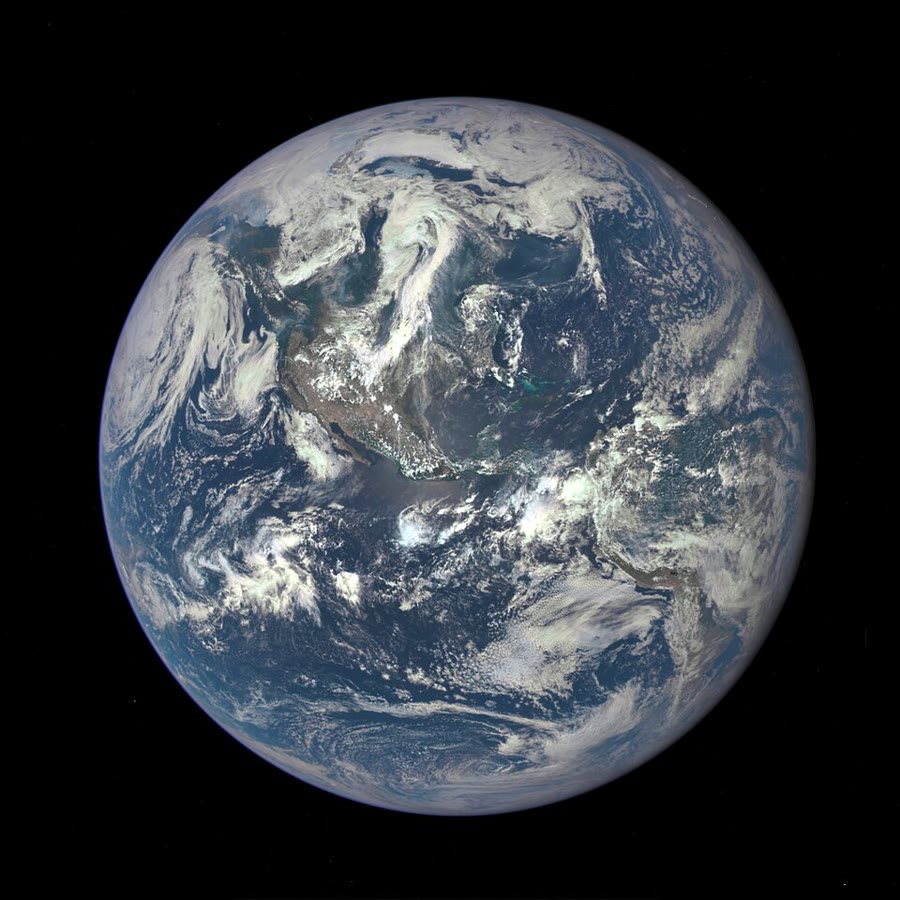
\includegraphics[width=0.55\linewidth]{images/book3/b1-epic-earth.jpg}

{\small De volledige zonverlichte kant van de aarde, gefotografeerd op 6 juli 2015 door een camera aan boord van het Deep Space Climate Observatory, op anderhalf miljoen kilometer afstand; Noord- en Midden-Amerika liggen in het midden, met de turquoise ondiepe zeeën van de Caraïben. Twee weken na de zomerzonnewende wordt de Arctis, bovenaan, de hele dag door verlicht. De heldere wolken kaatsen een groot deel van het licht dat hen bereikt terug; de blauwachtige tint is zonlicht dat door de moleculen van de lucht wordt verstrooid. (NASA Goddard Space Flight Center, publiek domein, via Wikimedia Commons.)}
\label{fig:b1:radiation-heat-transport:epic}
\end{omfigure}
% ledger: commons:epic-earth (polar day: figdata/bachelor-1/insolation.py)

\begin{recall}
\Cref{ch:b1:spherical-astronomy} definieerde de \omterm{def:b1:spherical-astronomy:insolation}{insolatie}, het vermogen van het zonlicht dat per vierkante meter van een horizontaal oppervlak aan de top van de atmosfeer wordt ontvangen, $I = S_0(a/r)^2\sin h_\odot$ zolang de zon boven de horizon staat, met $S_0 = \qty{1361}{W.m^{-2}}$ op de gemiddelde afstand $a$; gaf de hoogte van de zon boven de horizon uit haar \omterm{def:b1:spherical-astronomy:equatorial}{uurhoek} $H$, haar \omterm{def:b1:spherical-astronomy:equatorial}{declinatie} $\delta$ en de \omterm{def:b1:spherical-astronomy:geographic}{breedtegraad} $\varphi$, $\sin h_\odot = \sin\varphi\sin\delta + \cos\varphi\cos\delta\cos H$; en de \omterm{def:b1:spherical-astronomy:equatorial}{uurhoek} $H_0$ van zonsondergang, $\cos H_0 = -\tan\varphi\tan\delta$ (\cref{prop:b1:spherical-astronomy:rising}). \Cref{ch:b1:comparative-planetology} definieerde de \omterm{def:b1:comparative-planetology:albedo}{Bond-albedo} van een planeet en haar \omterm{def:b1:comparative-planetology:equilibrium-temperature}{evenwichtstemperatuur}. De natuurkundeboeken geven de kwadratenwet voor licht, de straling van een zwart lichaam, $\sigma T^4$ per vierkante meter met $\sigma = \qty{5.670e-8}{W.m^{-2}.K^{-4}}$ (Stefan--Boltzmann), en de latente warmte van een faseovergang. Boek~2 toonde dat de aarde gemiddeld een kwart van de zonneconstante onderschept, tekende de globale energiebalans van de aarde en controleerde dat zij in evenwicht is, en beschreef het poolwaartse warmtetransport met woorden.
% ledger: earth:TSI, const:sigma, ipcc:budget-toa
\end{recall}

\section{Insolatie met breedtegraad en seizoen}\label{sec:b1:radiation-heat-transport:insolation}

De momentane \omterm{def:b1:spherical-astronomy:insolation}{insolatie} verandert van minuut tot minuut terwijl de zon de hemel doorkruist. Voor het klimaat telt haar som over een dag.

\begin{definition}[Dagelijks gemiddelde insolatie]\label{def:b1:radiation-heat-transport:daily-insolation}
De \emph{dagelijks gemiddelde insolatie}\index{dagelijks gemiddelde insolatie} $\bar Q$ op een \omterm{def:b1:spherical-astronomy:geographic}{breedtegraad} op een gegeven dag is de momentane \omterm{def:b1:spherical-astronomy:insolation}{insolatie} gemiddeld over de 24 uur van die dag, nachten inbegrepen, waarbij de \omterm{def:b1:spherical-astronomy:equatorial}{declinatie} van de zon en haar afstand op hun waarden voor de dag worden gehouden. Het is een vermogen per vierkante meter horizontaal oppervlak aan de top van de atmosfeer, in \unit{W.m^{-2}}.
\end{definition}

Het vasthouden van $\delta$ en $r$ voor een dag is onschadelijk: de \omterm{def:b1:spherical-astronomy:equatorial}{declinatie} verandert met hoogstens \ang{0.4} per dag, en de afstand met minder dan \qty{0.03}{\percent}.
% ledger: earth:obliquity, earth:ecc (computed in figdata/bachelor-1/insolation.py)

\begin{theorem}[Dagelijks gemiddelde insolatie]\label{thm:b1:radiation-heat-transport:daily}
Op \omterm{def:b1:spherical-astronomy:geographic}{breedtegraad} $\varphi$, op een dag waarop de \omterm{def:b1:spherical-astronomy:equatorial}{declinatie} van de zon $\delta$ is en haar afstand $r$,
\[
  \bar Q = \frac{S_0}{\pi}\left(\frac{a}{r}\right)^{2}
  \bigl(h_0\sin\varphi\sin\delta + \cos\varphi\cos\delta\sin h_0\bigr),
\]
waarin $h_0 \in [0, \pi]$ de \omterm{def:b1:spherical-astronomy:equatorial}{uurhoek} van zonsondergang is in radialen: $\cos h_0 =
-\tan\varphi\tan\delta$ wanneer $|\tan\varphi\tan\delta| \le 1$; $h_0 = \pi$ in de polaire dag ($\tan\varphi\tan\delta > 1$); $h_0 = 0$, en $\bar Q = 0$, in de polaire nacht ($\tan\varphi\tan\delta < -1$).
\end{theorem}

\begin{proof}
De \omterm{def:b1:spherical-astronomy:equatorial}{uurhoek} $H$ loopt in een dag gelijkmatig door $2\pi$, dus is het gemiddelde over de dag het gemiddelde over $H \in [-\pi, \pi]$. De zon staat boven de horizon voor $-h_0 < H < h_0$, waar $\sin h_\odot > 0$, en de \omterm{def:b1:spherical-astronomy:insolation}{insolatie} is anders nul. Dus
\[
  \bar Q = \frac{1}{2\pi}\int_{-h_0}^{h_0} S_0\left(\frac{a}{r}\right)^{2}
  \bigl(\sin\varphi\sin\delta + \cos\varphi\cos\delta\cos H\bigr)\,\mathrm dH ,
\]
wat gelijk is aan $(S_0/2\pi)(a/r)^2\bigl(2h_0\sin\varphi\sin\delta +
2\cos\varphi\cos\delta\sin h_0\bigr)$.
De grenzen komen uit \cref{prop:b1:spherical-astronomy:rising}: de hoogte is nul wanneer $\cos H = -\tan\varphi\tan\delta$. Als dat getal in absolute waarde groter dan 1 is, gaat de zon nooit over de horizon: wanneer $\tan\varphi\tan\delta > 1$, is de integrand positief voor elke $H$ en loopt de integraal over de hele dag, $h_0 = \pi$; wanneer $\tan\varphi\tan\delta < -1$, is zij voor elke $H$ negatief en komt de zon nooit op.
\end{proof}

Twee bijzondere gevallen zijn goed om uit het hoofd te kennen. Aan de evenaar is $\varphi = 0$ en $h_0 = \pi/2$, wat het seizoen ook is:
\[
  \bar Q_\text{evenaar} = \frac{S_0}{\pi}\left(\frac{a}{r}\right)^{2}\cos\delta ,
\]
het grootst bij de equinoxen, $S_0/\pi = \qty{433.2}{W.m^{-2}}$ op de gemiddelde afstand. Bij een pool in haar zomer is $h_0 = \pi$ en $\varphi = \pi/2$: $\bar Q_\text{pool} =
S_0(a/r)^2\sin\delta$, de zon die de hemel rondgaat op een constante hoogte gelijk aan de \omterm{def:b1:spherical-astronomy:equatorial}{declinatie}.
% ledger: earth:TSI

\begin{proposition}[De poolzomer]\label{prop:b1:radiation-heat-transport:polar-summer}
Op een dag met \omterm{def:b1:spherical-astronomy:equatorial}{declinatie} $\delta > 0$ overtreft de \omterm{def:b1:radiation-heat-transport:daily-insolation}{dagelijks gemiddelde insolatie} aan de Noordpool die aan de evenaar dan en slechts dan wanneer $\pi\tan\delta > 1$, dat wil zeggen $\delta >
\ang{17.66}$. Op de zomerzonnewende van juni is $\delta = \ang{23.44}$, de verhouding is $\pi\tan
\delta = 1.362$.
\end{proposition}

\begin{proof}
De twee bijzondere gevallen hierboven delen de factor $(S_0/\pi)(a/r)^2$; hun verhouding is $\pi\sin\delta/\cos\delta = \pi\tan\delta$, die groter is dan 1 wanneer $\tan\delta >
1/\pi$, $\delta > \arctan(1/\pi) = \ang{17.66}$. Met de scheefstand, $\pi\tan\ang{23.44} = 1.362$.
\end{proof}
% ledger: earth:obliquity

Met de baan van de aarde valt de zomerzonnewende van juni nabij het aphelium, $(a/r)^2 = 0.968$: de Noordpool ontvangt dan \qty{524}{W.m^{-2}} als dagelijks gemiddelde, de evenaar \qty{385}{W.m^{-2}}. Zes maanden later ontvangt de Zuidpool, nabij het perihelium, \qty{559}{W.m^{-2}}, \qty{6.7}{\percent} meer dan de Noordpool in haar zomer had: de verhouding is precies die van de twee waarden van $(a/r)^2$. De figuur hieronder toont $\bar Q$ over een heel jaar. De maxima liggen aan de polen op de zonnewendes; de donkere wiggen zijn de poolnachten, begrensd door de \omterm{def:b1:spherical-astronomy:geographic}{breedtegraad} $\ang{90} -
|\delta|$; het subzonnepunt, waar de zon om het middaguur boven het hoofd staat, beweegt tussen de tropen met de \omterm{def:b1:spherical-astronomy:equatorial}{declinatie}.
% ledger: earth:TSI, earth:ecc, earth:obliquity, nasa:earth-perihelion-longitude, usno:seasons-2026 (computed in figdata/bachelor-1/insolation.py)

\begin{omfigure}
\begin{tikzpicture}
\begin{axis}[omrecord, width=0.8\linewidth, height=6.4cm, view={0}{90},
  xmin=0, xmax=365, ymin=-90, ymax=90, xlabel={dag van het jaar (vanaf 1 januari)},
  ylabel={breedtegraad (\unit{\degree})}, xtick={0,60,...,360}, ytick={-90,-60,...,90},
  colormap/viridis, colorbar, point meta min=0, point meta max=560,
  colorbar style={ylabel={$\bar Q$ (\unit{W.m^{-2}})}, ytick={0,100,...,500}, width=0.3cm},
  axis on top, grid=none]
% figdata/bachelor-1/insolation.py; ledger: earth:TSI, earth:ecc, earth:obliquity, nasa:earth-perihelion-longitude, usno:tropical-year, usno:seasons-2026
\addplot3[surf, shader=interp, mesh/ordering=y varies, mesh/rows=73]
  table[x=day, y=lat, z=Q] {figdata/out/bachelor-1-insolation-grid.dat};
\addplot3[white, dashed, line width=0.8pt] table[x=day, y=decl, z expr=600] {figdata/out/bachelor-1-insolation-sun.dat};
\addplot3[white, line width=0.6pt, unbounded coords=jump] table[x=day, y=night_n, z expr=600] {figdata/out/bachelor-1-insolation-sun.dat};
\addplot3[white, line width=0.6pt, unbounded coords=jump] table[x=day, y=night_s, z expr=600] {figdata/out/bachelor-1-insolation-sun.dat};
\node[font=\scriptsize, text=white] at (axis cs:28,81,700) {polaire nacht};
\node[font=\scriptsize, text=white] at (axis cs:172,-81,700) {polaire nacht};
\node[font=\scriptsize, text=white, anchor=south] at (axis cs:172,26,700) {subzonnebreedte};
\end{axis}
\end{tikzpicture}

{\small \omterm{def:b1:radiation-heat-transport:daily-insolation}{Dagelijks gemiddelde insolatie} aan de top van de atmosfeer tegen de dag van het jaar en de \omterm{def:b1:spherical-astronomy:geographic}{breedtegraad}, uit \cref{thm:b1:radiation-heat-transport:daily} met $S_0 = \qty{1361}{W.m^{-2}}$ en de baan van de aarde. Gestreept: de subzonnebreedte, gelijk aan de \omterm{def:b1:spherical-astronomy:equatorial}{declinatie}; vol: de randen van de poolnachten. De zomerpolen ontvangen meer dan elke andere plaats op de aarde; de zuidelijke zomer, nabij het perihelium, is de helderste van de twee.}
\label{fig:b1:radiation-heat-transport:matrix}
\end{omfigure}
% ledger: earth:TSI, earth:ecc, earth:obliquity, nasa:earth-perihelion-longitude, usno:seasons-2026

Het jaargemiddelde van $\bar Q$ geeft de jaargemiddelde \omterm{def:b1:spherical-astronomy:insolation}{insolatie} van elke \omterm{def:b1:spherical-astronomy:geographic}{breedtegraad} (figuur hieronder): \qty{415.6}{W.m^{-2}} aan de evenaar, \qty{328.3}{W.m^{-2}} op \ang{40}, \qty{172.4}{W.m^{-2}} aan elke pool. De poolzomer is intens maar de poolwinter donker, en over een jaar ontvangt de evenaar \num{2.41} keer zoveel als een pool. De kromme is in beide hemisferen dezelfde, al is de zuidelijke zomer helderder; \cref{exo:b1:radiation-heat-transport:10} laat zien waarom.
% ledger: earth:TSI, earth:ecc, earth:obliquity (computed in figdata/bachelor-1/insolation.py)

\begin{omfigure}
\begin{tikzpicture}
\begin{axis}[omrecord, width=0.8\linewidth, height=5.6cm, xmin=-90, xmax=90, ymin=0, ymax=600,
  xlabel={breedtegraad (\unit{\degree})}, ylabel={$\bar Q$ (\unit{W.m^{-2}})},
  xtick={-90,-60,...,90}, ytick={0,100,...,600}]
% figdata/bachelor-1/insolation.py; ledger: earth:TSI, earth:ecc, earth:obliquity, nasa:earth-perihelion-longitude
\addplot[omThm, line width=0.8pt] table[x=lat, y=Q_jun] {figdata/out/bachelor-1-insolation-annual.dat};
\addplot[omDef, line width=0.8pt] table[x=lat, y=Q_dec] {figdata/out/bachelor-1-insolation-annual.dat};
\addplot[black, line width=1.1pt] table[x=lat, y=Q_ann] {figdata/out/bachelor-1-insolation-annual.dat};
\addplot[black!60, dashed, domain=-90:90] {340.30};
\node[font=\scriptsize, text=omThm, anchor=west] at (axis cs:50,540) {junizonnewende};
\node[font=\scriptsize, text=omDef, anchor=east] at (axis cs:-50,575) {decemberzonnewende};
\node[font=\scriptsize, anchor=north] at (axis cs:-72,160) {jaargemiddelde};
\node[font=\scriptsize, text=black!60, anchor=south west] at (axis cs:-88,342) {wereldgemiddelde};
\end{axis}
\end{tikzpicture}

{\small \omterm{def:b1:radiation-heat-transport:daily-insolation}{Dagelijks gemiddelde insolatie} tegen \omterm{def:b1:spherical-astronomy:geographic}{breedtegraad} bij de twee zonnewendes, en haar jaargemiddelde (zwart). Het jaargemiddelde overtreft het wereldgemiddelde, \qty{340.3}{W.m^{-2}} (gestreept), tussen \ang{37} Z en \ang{37} N, op \qty{60}{\percent} van het aardoppervlak.}
\label{fig:b1:radiation-heat-transport:annual}
\end{omfigure}
% ledger: earth:TSI, earth:ecc, earth:obliquity (computed in figdata/bachelor-1/insolation.py)

\begin{proposition}[Het wereldgemiddelde]\label{prop:b1:radiation-heat-transport:global}
Op elk ogenblik is de \omterm{def:b1:spherical-astronomy:insolation}{insolatie} gemiddeld over de hele bol $\tfrac14
S_0(a/r)^2$. Gemiddeld over het jaar ook, is zij $S_0/(4\sqrt{1 - e^2})$, waarin $e$ de excentriciteit van de baan is: \qty{340.30}{W.m^{-2}} voor de aarde, binnen \qty{0.02}{\percent} van $S_0/4 = \qty{340.25}{W.m^{-2}}$.
\end{proposition}

\begin{proof}
De aarde, met straal $R$, onderschept het zonlicht dat een schijf van oppervlakte $\pi
R^2$ kruist, een vermogen $S_0(a/r)^2\pi R^2$, dat op de dagkant valt; verspreid over het hele oppervlak $4\pi R^2$ geeft dit het eerste resultaat. Het tijdgemiddelde van $(a/r)^2$ over de baan is $1/\sqrt{1-e^2}$
(\cref{exo:b1:radiation-heat-transport:11}).
\end{proof}
% ledger: earth:TSI, earth:ecc

\section{Geabsorbeerde en uitgezonden straling}\label{sec:b1:radiation-heat-transport:toa}

Van het zonlicht dat een \omterm{def:b1:spherical-astronomy:geographic}{breedtegraad} ontvangt, wordt een deel rechtstreeks teruggekaatst door wolken, sneeuw, ijs, woestijn en, in mindere mate, zee; de rest wordt geabsorbeerd, in de lucht en aan het oppervlak. Zij verliest ook energie door infrarode straling naar de ruimte uit te zenden, dag en nacht.

\begin{definition}[Uitgaande langgolvige straling]\label{def:b1:radiation-heat-transport:olr}
De \emph{uitgaande langgolvige straling}\index{uitgaande langgolvige straling} (OLR) is het vermogen van infrarode straling die de top van de atmosfeer naar de ruimte verlaat, per vierkante meter. De \emph{emissietemperatuur}\index{emissietemperatuur} $T_e$ is de temperatuur van een zwart lichaam dat hetzelfde vermogen zou uitzenden: $\sigma T_e^4 = \text{OLR}$.
\end{definition}

De OLR komt deels van het oppervlak, door de lucht heen waar die doorzichtig is voor infrarood, en deels van de lucht en de wolkentoppen hoger op. De \omterm{def:b1:radiation-heat-transport:olr}{emissietemperatuur} is een eigenschap van de straling, niet de temperatuur van een bepaald niveau: zij is lager dan die van de grond eronder, omdat de uitzendende lagen kouder zijn.
% ledger: ipcc:budget-surface, ipcc:budget-toa

\begin{definition}[Netto straling; stralingsoverschot en -tekort]\label{def:b1:radiation-heat-transport:net-radiation}
De \emph{netto straling}\index{netto straling} aan de top van de atmosfeer is
\[
  R = \underbrace{(1 - \alpha)\,\bar Q}_{\text{geabsorbeerde zon}} - \text{OLR},
\]
waarin $\alpha$ de lokale albedo is, het deel van het binnenkomende zonlicht dat naar de ruimte wordt teruggekaatst; alle drie grootheden zijn jaargemiddelden op één \omterm{def:b1:spherical-astronomy:geographic}{breedtegraad}. Een \omterm{def:b1:spherical-astronomy:geographic}{breedtegraad} waar $R > 0$ heeft een \emph{stralingsoverschot}\index{stralingsoverschot}; een waar $R < 0$
heeft een \emph{stralingstekort}\index{stralingstekort}.
\end{definition}

Over de hele aarde moet de \omterm{def:b1:radiation-heat-transport:net-radiation}{netto straling} bijna nul gemiddeld zijn, want de planeet warmt noch koelt met meer dan enkele tienden van een watt per vierkante meter: de jongste beoordeling geeft de onbalans op \qty{0.7}{W.m^{-2}}, op een binnenkomende \qty{340}{W.m^{-2}} waarvan \qty{100}{W.m^{-2}} worden teruggekaatst (een wereldwijde albedo van \num{0.294}) en \qty{239}{W.m^{-2}} als infrarood vertrekken.
% ledger: ipcc:budget-toa, earth:albedo

De zonale profielen van dit hoofdstuk komen uit een reanalyse: een weersvoorspellingssysteem dat over de voorbije decennia is gedraaid, dat de waarnemingen van elke dag assimileert en een volledige, consistente toestand van de atmosfeer geeft. De hier gebruikte reanalyse, vanaf 1948, geeft maandgemiddelden op een rooster van 94 breedtegraden en 192 lengtegraden; dit hoofdstuk gebruikt haar gemiddelden over 1991--2020. Haar stralingsfluxen zijn modeluitvoer, voorspellingen die door de waarnemingen worden beperkt. De figuur hieronder toont hun zonale gemiddelden tegen $\sin\varphi$, zodat gelijke breedten op de as gelijke oppervlakken op de bol zijn.
% ledger: psl:ncep-r1, kalnay96:reanalysis, data:b3-ncep

\begin{omfigure}
\begin{tikzpicture}
\begin{axis}[omrecord, width=0.8\linewidth, height=6cm, xmin=-1, xmax=1, ymin=0, ymax=320,
  xlabel={breedtegraad (\unit{\degree}, as in $\sin\varphi$)}, ylabel={flux (\unit{W.m^{-2}})},
  xtick={-0.866,-0.5,0,0.5,0.866}, xticklabels={60 Z,30 Z,0,30 N,60 N},
  ytick={0,50,...,300}]
% figdata/bachelor-1/energy_balance.py; ledger: data:b3-ncep, psl:ncep-r1
\addplot[name path=asr, omProp, line width=1pt] table[x expr={sin(\thisrow{lat})}, y=asr] {figdata/out/bachelor-1-energy_balance-toa.dat};
\addplot[name path=olr, omThm, line width=1pt] table[x expr={sin(\thisrow{lat})}, y=olr] {figdata/out/bachelor-1-energy_balance-toa.dat};
\addplot[omProp!25] fill between[of=asr and olr, split, every segment no 1/.style={omDef!18}, every segment no 2/.style={omProp!30}, every segment no 3/.style={omDef!18}];
\node[font=\scriptsize, text=omProp!80!black] at (axis cs:-0.55,300) {geabsorbeerde zon};
\node[font=\scriptsize, text=omThm] at (axis cs:-0.2,226) {OLR};
\node[font=\scriptsize] at (axis cs:0,262) {overschot};
\node[font=\scriptsize] at (axis cs:0.86,178) {tekort};
\node[font=\scriptsize] at (axis cs:-0.86,178) {tekort};
\end{axis}
\end{tikzpicture}

{\small Zonaal en jaargemiddeld geabsorbeerd zonlicht (oranje) en \omterm{def:b1:radiation-heat-transport:olr}{uitgaande langgolvige straling} (rood) aan de top van de atmosfeer, uit de NCEP-NCAR-reanalyse 1, gemiddelden 1991--2020 (gegevens verstrekt door de NOAA PSL, Boulder, Colorado, VS, via hun website op https://psl.noaa.gov). Gearceerd: het \omterm{def:b1:radiation-heat-transport:net-radiation}{stralingsoverschot} van de lage breedtegraden en de \omterm{def:b1:radiation-heat-transport:net-radiation}{stralingstekorten} van de hoge breedtegraden.}
\label{fig:b1:radiation-heat-transport:toa}
\end{omfigure}
% ledger: data:b3-ncep, psl:ncep-r1, kalnay96:reanalysis

De twee kromme hebben zeer verschillende vormen. Het geabsorbeerde zonlicht daalt van \qty{288}{W.m^{-2}} nabij de evenaar tot \qty{76}{W.m^{-2}} op \ang{81} N, met een factor van \num{3.8}: de \omterm{def:b1:spherical-astronomy:insolation}{insolatie} daalt, en de albedo stijgt van \num{0.31} tot \num{0.57}, met de lage zon, de sneeuw en het zee-ijs. De OLR daalt slechts van \qty{245}{W.m^{-2}} tot \qty{192}{W.m^{-2}}, met een factor van \num{1.27}; de emissietemperaturen zijn \qty{256}{K} en \qty{241}{K}. De OLR is zelfs iets lager aan de evenaar, \qty{245}{W.m^{-2}}, dan nabij \ang{20}, \qty{269}{W.m^{-2}}: de wolken van de equatoriale regengordel reiken hoog en hun koude toppen zenden weinig uit, terwijl de helderdere subtropische luchten meer infrarood laten ontsnappen. Waar het geabsorbeerde zonlicht de OLR overtreft, heeft de \omterm{def:b1:spherical-astronomy:geographic}{breedtegraad} een overschot.
% ledger: data:b3-ncep (values computed in figdata/bachelor-1/energy_balance.py)

\begin{example}[Het wereldwijde budget van de reanalyse]\label{ex:b1:radiation-heat-transport:global}
Over de hele bol gemiddeld ontvangt de reanalyse \qty{341.9}{W.m^{-2}}, kaatst zij \qty{117.0}{W.m^{-2}} terug (een albedo van \num{0.342}), absorbeert zij \qty{224.8}{W.m^{-2}} en zendt zij \qty{237.7}{W.m^{-2}} uit: een \omterm{def:b1:radiation-heat-transport:net-radiation}{netto straling} van \qty{-12.9}{W.m^{-2}}. De OLR ligt binnen \qty{1.3}{W.m^{-2}} van de beoordeelde \qty{239}{W.m^{-2}}, maar de terugkaatsing is \qty{17}{W.m^{-2}} groter dan de beoordeelde \qty{100}{W.m^{-2}}. Een werkelijke onbalans van deze omvang zou de aarde met \qty{6.6}{PW} doen afkoelen; het is een fout van het model, geen eigenschap van de aarde, en het transport hieronder wordt berekend na aftrek van het wereldgemiddelde.
% ledger: data:b3-ncep, ipcc:budget-toa (computed in figdata/bachelor-1/energy_balance.py)
\end{example}

\section{Meridionaal warmtetransport}\label{sec:b1:radiation-heat-transport:transport}

\begin{definition}[Meridionaal warmtetransport]\label{def:b1:radiation-heat-transport:mht}
Het \emph{meridionale warmtetransport}\index{meridionale warmtetransport} $T(\varphi)$
over de parallel van \omterm{def:b1:spherical-astronomy:geographic}{breedtegraad} $\varphi$ is de energie die per tijdseenheid noordwaarts over die parallel wordt meegevoerd, door atmosfeer en oceaan samen, in het jaargemiddelde. Het wordt positief noordwaarts geteld en gemeten in petawatt
(\qty{1}{PW} = \qty{e15}{W}).
\end{definition}

\begin{proposition}[Transport uit de netto straling]\label{prop:b1:radiation-heat-transport:mht}
Als de energie die in elke breedtegraadband is opgeslagen van jaar tot jaar niet verandert, dan geldt voor een aarde met straal $a_\oplus$,
\[
  T(\varphi) = 2\pi a_\oplus^2\int_{-\pi/2}^{\varphi} R(\varphi')\cos\varphi'\,
  \mathrm d\varphi' = -2\pi a_\oplus^2\int_{\varphi}^{\pi/2} R(\varphi')\cos
  \varphi'\,\mathrm d\varphi' ,
\]
en $T$ is extreem op de breedtegraden waar $R$ van teken verandert.
\end{proposition}

\begin{proof}
Neem de poolkap ten zuiden van de parallel $\varphi$ als controlevolume, van de bodem van de oceaan tot de top van de atmosfeer (figuur hieronder). Energie komt erin of verlaat het op maar twee manieren: als straling aan de top, een netto vermogen $\int R\,\mathrm dA$, en door het transport over zijn rand, $-T(\varphi)$ (een noordwaarts transport verlaat de zuidelijke kap). De band tussen $\varphi'$ en $\varphi' + \mathrm d\varphi'$ heeft oppervlakte $\mathrm dA = 2\pi a_\oplus\cos\varphi'
\cdot a_\oplus\,\mathrm d\varphi'$. Zonder verandering van opslag is de som nul:
$\int_{-\pi/2}^{\varphi} R\,2\pi a_\oplus^2\cos\varphi'\,\mathrm d\varphi' -
T(\varphi) = 0$. Toegepast op de hele aarde ($\varphi = \pi/2$, geen rand) geeft dezelfde balans $\int R\,\mathrm dA = 0$ over de bol, vandaar de tweede vorm. Door te differentiëren geldt $T'(\varphi) = 2\pi a_\oplus^2 R(\varphi)\cos\varphi$, wat nul is waar $R$ van teken verandert.
\end{proof}
% ledger: earth:Rmean

\begin{omfigure}
\begin{tikzpicture}[>={Stealth[length=2mm]}, font=\scriptsize]
  \def\R{2.0}
  \def\ph{40}
  \fill[omDef!12] ({-\R*cos(\ph)},{\R*sin(\ph)}) arc[start angle=180-\ph, end angle=\ph, radius=\R]
     -- ({\R*cos(\ph)},{\R*sin(\ph)}) arc[start angle=0, end angle=-180, x radius={\R*cos(\ph)}, y radius={0.25*\R*cos(\ph)}] -- cycle;
  \draw[thick] (0,0) circle (\R);
  \draw[black!40] (-\R,0) arc[start angle=180, end angle=360, x radius=\R, y radius={0.25*\R}];
  \draw[black!40, dashed] (\R,0) arc[start angle=0, end angle=180, x radius=\R, y radius={0.25*\R}];
  \draw[omDef, thick] ({-\R*cos(\ph)},{\R*sin(\ph)}) arc[start angle=180, end angle=360, x radius={\R*cos(\ph)}, y radius={0.25*\R*cos(\ph)}];
  \draw[omDef, thick, dashed] ({\R*cos(\ph)},{\R*sin(\ph)}) arc[start angle=0, end angle=180, x radius={\R*cos(\ph)}, y radius={0.25*\R*cos(\ph)}];
  \node[anchor=west, black!60] at (\R+0.05,0) {evenaar};
  \node[anchor=west, omDef] at ({\R*cos(\ph)+0.1},{\R*sin(\ph)}) {parallel $\varphi$};
  \foreach \x in {-0.55,0.55} \draw[->, very thick, omProp] (\x,{\R*sin(\ph)-0.75}) -- (\x,{\R*sin(\ph)-0.1});
  \node[omProp!80!black, anchor=east] at ({-\R-0.1},{\R*sin(\ph)-0.4}) {$T(\varphi)$ steekt de rand over};
  \foreach \a in {65,90,115} {
    \draw[->, omThm, decorate, decoration={snake, amplitude=0.6mm, segment length=2mm, post length=1.5mm}]
      ({(\R+0.05)*cos(\a)},{(\R+0.05)*sin(\a)}) -- ({(\R+0.75)*cos(\a)},{(\R+0.75)*sin(\a)});
  }
  \node[omThm, anchor=south] at (0,\R+0.8) {nettostraling $R < 0$ boven de kap};
\end{tikzpicture}

{\small Het controlevolume van \cref{prop:b1:radiation-heat-transport:mht}, getekend voor de kap ten noorden van de parallel $\varphi$ (gearceerd): in een stationaire toestand is wat de kap door straling aan de top van de atmosfeer verliest (rood) gelijk aan wat de atmosfeer en de oceaan over haar rand aanvoeren (oranje).}
\label{fig:b1:radiation-heat-transport:cap}
\end{omfigure}

Toegepast op de reanalyse, met het wereldgemiddelde van \qty{-12.9}{W.m^{-2}} afgetrokken van $R$ op elke \omterm{def:b1:spherical-astronomy:geographic}{breedtegraad}, geeft de propositie de kromme hieronder. Het transport is noordwaarts op het noordelijk halfrond en zuidwaarts op het zuidelijke, altijd naar de pool toe. Het bereikt een piek van \qty{4.1}{PW} nabij \ang{38} N en \qty{4.5}{PW} nabij \ang{32} S, waar $R$, verminderd met het wereldgemiddelde, van teken verandert; over \ang{40} N is het \qty{4.11}{PW}. Het is klein aan de evenaar, waar het overschot van elk halfrond naar de eigen pool wordt geëxporteerd.
% ledger: data:b3-ncep (computed in figdata/bachelor-1/energy_balance.py)

\begin{omfigure}
\begin{tikzpicture}
\begin{axis}[omrecord, width=0.8\linewidth, height=6cm, xmin=-90, xmax=90, ymin=-5.5, ymax=6.4,
  xlabel={breedtegraad (\unit{\degree})}, ylabel={noordwaarts transport (\unit{PW})},
  xtick={-90,-60,...,90}, ytick={-4,-2,...,4}]
% figdata/bachelor-1/energy_balance.py; ledger: data:b3-ncep, trenberth:transport
\addplot[black!40, domain=-90:90] {0};
\addplot[black, line width=1.1pt] table[x=lat, y=T_PW] {figdata/out/bachelor-1-energy_balance-transport.dat};
\addplot[omMeth, dashed, line width=0.9pt] table[x=lat, y=T_PW] {figdata/out/bachelor-1-energy_balance-latent.dat};
\addplot[only marks, mark=square*, mark size=2pt, omThm] coordinates {(43,5.0)};
\node[font=\scriptsize, anchor=east] at (axis cs:28,4.4) {totaal};
\node[font=\scriptsize, text=omMeth, anchor=north] at (axis cs:42,0.9) {latente warmte};
\node[font=\scriptsize, text=omThm, anchor=south] at (axis cs:43,5.2) {alleen atmosfeer (Trenberth en Caron)};
\end{axis}
\end{tikzpicture}

{\small Het \omterm{def:b1:radiation-heat-transport:mht}{meridionale warmtetransport} dat uit de \omterm{def:b1:radiation-heat-transport:net-radiation}{netto straling} van de reanalyse volgt (zwart) en zijn latente-warmtedeel (gestreept groen, uit de verdamping en de neerslag, \cref{sec:b1:radiation-heat-transport:latent}); NCEP-NCAR-reanalyse 1, gemiddelden 1991--2020, gegevens verstrekt door de NOAA PSL. Vierkant: de piek van het atmosferisch transport alleen, in een schatting die door satellietmetingen van de straling is beperkt, \qty{5.0}{PW} op \ang{43} N (Trenberth en Caron, 2001).}
\label{fig:b1:radiation-heat-transport:transport}
\end{omfigure}
% ledger: data:b3-ncep, psl:ncep-r1, trenberth:transport

De vierkant op de figuur is een waarschuwing. Een studie van de jaren 1985--1989, toen een satellietexperiment de straling aan de top van de atmosfeer betrouwbaar mat, berekende het transport van de atmosfeer uit de winden, temperaturen en vochtigheid van twee reanalyses: de atmosfeer alleen draagt \qty{5.0}{PW} op \ang{43} N, meer dan de \qty{4.0}{PW} van deze reanalyse voor atmosfeer en oceaan samen. Dezelfde studie vond dat de door het model voortgebrachte fluxen van de reanalyse slechter overeenkomen met onafhankelijke schattingen van de oceaan dan fluxen die uit de waarnemingen zijn afgeleid. Met het wereldgemiddelde afgetrokken, hangt het transport alleen af van hoe $R$ met de \omterm{def:b1:spherical-astronomy:geographic}{breedtegraad} varieert, en de \omterm{def:b1:radiation-heat-transport:net-radiation}{netto straling} van deze reanalyse varieert te weinig van de tropen naar de polen. De vorm van de kromme, haar pieken in de middelbreedten en haar bijna-symmetrie, kunnen worden vertrouwd; haar hoogte blijft minstens een vijfde te laag.
% ledger: trenberth:transport, tc01:method, data:b3-ncep (computed in figdata/bachelor-1/energy_balance.py)

Wie draagt de warmte? Dezelfde studie vindt dat de oceaan meer draagt dan de atmosfeer alleen tussen de evenaar en \ang{17} N; op \ang{35}, waar het totale transport in elk halfrond piekt, draagt de atmosfeer \qty{78}{\percent} ervan in het noorden en \qty{92}{\percent} in het zuiden. Het aandeel van de oceaan is het onderwerp van \cref{ch:b1:ocean-circulation}, dat van de atmosfeer van \cref{ch:b1:atmospheric-circulation}.
% ledger: trenberth:transport

\begin{method}[Transport uit zonale banden]\label{met:b1:radiation-heat-transport:bands}
\begin{enumerate}
  \item Verdeel het gebied tussen de \omterm{def:b1:spherical-astronomy:geographic}{breedtegraad} van belang en de pool in banden; neem voor elk de gemiddelde \omterm{def:b1:spherical-astronomy:insolation}{insolatie} $\bar Q_i$, albedo $\alpha_i$ en OLR$_i$.
  \item Bereken de \omterm{def:b1:radiation-heat-transport:net-radiation}{netto straling} van elke band, $R_i = (1 - \alpha_i)\bar Q_i -
        \text{OLR}_i$, en trek het wereldgemiddelde van $R$ af als het niet nul is.
  \item Bereken het oppervlak van elke band, $A_i = 2\pi a_\oplus^2(\sin\varphi_{i,2} -
        \sin\varphi_{i,1})$, met $a_\oplus = \qty{6371}{km}$.
  \item Het transport over de rand is het tegengestelde van het netto vermogen van de kap,
        $-\sum_i R_i A_i$, positief naar de pool; deel door \num{e15} voor
        petawatt.
\end{enumerate}
\end{method}
% ledger: earth:Rmean

\section{Latente en voelbare warmte}\label{sec:b1:radiation-heat-transport:latent}

Het aardoppervlak absorbeert het meeste zonlicht, maar de atmosfeer straalt het meeste infrarood naar de ruimte uit. Het oppervlak geeft energie aan de lucht op drie manieren: door zijn eigen infraroodstraling, door de lucht in contact ermee te verwarmen, en door water te laten verdampen, waarvan de latente warmte vrijkomt waar de damp condenseert. Die plaats kan duizenden kilometers verderop liggen: de latente warmte reist met de wind.

\begin{definition}[Latente en voelbare warmtefluxen; Bowen-verhouding]\label{def:b1:radiation-heat-transport:surface-fluxes}
De \emph{latente warmteflux}\index{latente warmteflux} $LE$ is het vermogen per vierkante meter dat het oppervlak door verdamping verliest: de verdampingssnelheid $E$, in
\unit{kg.m^{-2}.s^{-1}}, maal de latente warmte van verdamping $L$. De \emph{voelbare warmteflux}\index{voelbare warmteflux} $H$ is het vermogen per vierkante meter dat het oppervlak door geleiding en turbulentie aan de lucht doorgeeft, en die verwarmt. Beide worden positief naar boven geteld. Hun verhouding $B = H/LE$ is de \emph{Bowen-verhouding}\index{Bowen-verhouding}.
\end{definition}

Bij \qty{15}{\celsius} is $L = \qty{2.4655}{MJ.kg^{-1}}$. De \omterm{def:b1:radiation-heat-transport:surface-fluxes}{Bowen-verhouding} is klein boven de zee en boven nat land, waar water overvloedig is, en groot boven droog land. In de reanalyse is zij \num{0.09} aan de evenaar, \num{0.37} op \ang{25} N, de \omterm{def:b1:spherical-astronomy:geographic}{breedtegraad} van de grote hete woestijnen, en negatief op \ang{70} N, waar de sneeuw- en ijsoppervlakken in het jaargemiddelde kouder zijn dan de lucht erboven, zodat de voelbare \omterm{def:b1:heat-budget:heat-flow}{warmtestroom} naar beneden gaat. Over de hele aarde gemiddeld geeft de reanalyse $LE =
\qty{82.5}{W.m^{-2}}$ en $H = \qty{15.2}{W.m^{-2}}$, een \omterm{def:b1:radiation-heat-transport:surface-fluxes}{Bowen-verhouding} van \num{0.18}; de beoordeelde waarden zijn \qty{82}{W.m^{-2}} en \qty{21}{W.m^{-2}}, een verhouding van \num{0.26}.
% ledger: nist:water-latent, data:b3-ncep, ipcc:budget-surface (computed in figdata/bachelor-1/energy_balance.py)

Boek~2 zette de \omterm{def:b1:radiation-heat-transport:surface-fluxes}{latente warmteflux} om in een diepte van water dat elk jaar verdampt. De omgekeerde weg zet een regenval, die een regenmeter kan opvangen, om in een energieflux.

\begin{proposition}[Neerslag als energieflux]\label{prop:b1:radiation-heat-transport:rain}
Een neerslagsnelheid van \qty{1}{m} water per jaar geeft in de atmosfeer, waar de damp condenseerde, een gemiddeld vermogen van
\[
  \frac{\qty{1000}{kg.m^{-2}} \times \qty{2.4655e6}{J.kg^{-1}}}{\qty{3.156e7}{s}}
  = \qty{78.1}{W.m^{-2}} .
\]
\end{proposition}

\begin{proof}
Een laag water van \qty{1}{m} diep heeft een massa van \qty{1000}{kg} per vierkante meter. Het condenseren van de damp die daar ontstaat, geeft $1000L$ vrij; een jaar van \num{365.25} dagen duurt \qty{3.156e7}{s}.
\end{proof}
% ledger: nist:water-latent

\begin{example}[De watercyclus als energieflux]\label{ex:b1:radiation-heat-transport:rain}
De wereldwijde watercyclus brengt elk jaar \num{373000} kubieke kilometer regen en sneeuw naar de oceaan en \num{113000} naar het land: uitgespreid over de \qty{5.10e8}{km^2} van de aarde, \qty{0.953}{m} per jaar, wat \qty{74}{W.m^{-2}} vrijmaakt volgens \cref{prop:b1:radiation-heat-transport:rain}. De reanalyse regent \qty{2.82}{mm} per dag, \qty{1.03}{m} per jaar, \qty{80}{W.m^{-2}}. Beide liggen dicht bij de beoordeelde \omterm{def:b1:radiation-heat-transport:surface-fluxes}{latente warmteflux} van \qty{82}{W.m^{-2}}, waarvan het onzekerheidsbereik \qtyrange{72}{85}{W.m^{-2}} is: over de jaren komt het water dat verdampt weer naar beneden, en de latente warmte die van het oppervlak wordt genomen, wordt geheel aan de lucht gegeven.
% ledger: trenberth:water-cycle, earth:Rmean, data:b3-ncep, ipcc:budget-surface (computed in calc/ch27.py)
\end{example}

Het evenwicht geldt voor de hele bol, niet voor elke \omterm{def:b1:spherical-astronomy:geographic}{breedtegraad}, en het verschil is een transport (figuur hieronder). In de subtropen verdampt de zee meer water dan er daar valt: $LE$ overtreft $LP$, de latente warmte van de neerslag. De equatoriale regengordel en de middelbreedten ontvangen meer regen dan zij verdampen. Tussen beide wordt de damp door de wind meegevoerd, en met haar de latente warmte. Volgens het argument van \cref{prop:b1:radiation-heat-transport:mht}, toegepast op de integraal van $LE - LP$, draagt de reanalyse \qty{1.4}{PW} latente warmte noordwaarts over \ang{40} N, een derde van haar totale transport daar; het latente transport is gestreept getekend op de transportfiguur hierboven.
% ledger: data:b3-ncep (computed in figdata/bachelor-1/energy_balance.py)

\begin{omfigure}
\begin{tikzpicture}
\begin{axis}[omrecord, width=0.8\linewidth, height=6cm, xmin=-1, xmax=1, ymin=-60, ymax=200,
  xlabel={breedtegraad (\unit{\degree}, as in $\sin\varphi$)}, ylabel={flux (\unit{W.m^{-2}})},
  xtick={-0.866,-0.5,0,0.5,0.866}, xticklabels={60 Z,30 Z,0,30 N,60 N},
  ytick={-50,0,50,...,200}]
% figdata/bachelor-1/energy_balance.py; ledger: data:b3-ncep, nist:water-latent
\addplot[black!40, domain=-1:1] {0};
\addplot[omMeth, line width=1pt] table[x expr={sin(\thisrow{lat})}, y=lh] {figdata/out/bachelor-1-energy_balance-surface.dat};
\addplot[omDef, line width=1pt] table[x expr={sin(\thisrow{lat})}, y=lp] {figdata/out/bachelor-1-energy_balance-surface.dat};
\addplot[omThm, dashed, line width=0.9pt] table[x expr={sin(\thisrow{lat})}, y=sh] {figdata/out/bachelor-1-energy_balance-surface.dat};
\node[font=\scriptsize, text=omMeth, anchor=south] at (axis cs:-0.35,118) {$LE$};
\node[font=\scriptsize, text=omDef, anchor=south] at (axis cs:0.06,168) {$LP$};
\node[font=\scriptsize, text=omThm, anchor=south] at (axis cs:0.2,24) {$H$};
\end{axis}
\end{tikzpicture}

{\small Zonaal en jaargemiddelde van de \omterm{def:b1:radiation-heat-transport:surface-fluxes}{latente warmteflux} $LE$ (groen), van de latente warmte die bij de neerslag vrijkomt, $LP$ (blauw), en van de \omterm{def:b1:radiation-heat-transport:surface-fluxes}{voelbare warmteflux} $H$ (rood, gestreept), uit de NCEP-NCAR-reanalyse 1, gemiddelden 1991--2020 (gegevens verstrekt door de NOAA PSL). Waar $LE > LP$, in de subtropen, wordt waterdamp uitgevoerd; waar $LP > LE$, in de regengordels, wordt zij ingevoerd.}
\label{fig:b1:radiation-heat-transport:surface}
\end{omfigure}
% ledger: data:b3-ncep, psl:ncep-r1, nist:water-latent

\section{De energiebalans van het oppervlak}\label{sec:b1:radiation-heat-transport:surface}

De wereldwijde balans die in Boek~2 is getekend, kan worden gelezen als één vergelijking voor het oppervlak.

\begin{proposition}[Energiebalans van het oppervlak]\label{prop:b1:radiation-heat-transport:surface}
Zij $R_n$ de \omterm{def:b1:radiation-heat-transport:net-radiation}{netto straling} aan het oppervlak, geabsorbeerd zonlicht plus infrarood ontvangen van de lucht min het uitgezonden infrarood, en $G$ het vermogen per vierkante meter dat de bodem of de oceaan eronder in gaat. Dan geldt, per vierkante meter,
\[
  R_n = LE + H + G .
\]
In het wereldgemiddelde is $R_n = 160 + 342 - 398 = \qty{104}{W.m^{-2}}$, waarvan \qty{82}{W.m^{-2}} naar verdamping gaat, \qty{21}{W.m^{-2}} naar de \omterm{def:b1:radiation-heat-transport:surface-fluxes}{voelbare warmteflux}, en $G \approx \qty{1}{W.m^{-2}}$, binnen de afronding van de cijfers, naar de oceaan en de bodem.
\end{proposition}

\begin{proof}
Neem als systeem een dunne laag aan het oppervlak, zonder eigen warmtecapaciteit. Energie bereikt haar alleen als straling ($R_n$, netto) en verlaat haar alleen als de latente en \omterm{def:b1:radiation-heat-transport:surface-fluxes}{voelbare warmtefluxen} naar boven en de geleiding of menging naar beneden; de balans is de vergelijking. De getallen zijn de beoordeelde wereldgemiddelden.
\end{proof}
% ledger: ipcc:budget-surface

\begin{omfigure}
\begin{tikzpicture}[font=\scriptsize, >={Stealth[length=2.2mm, width=2mm]}, line width=1.3pt]
  \fill[omExo!35] (0,0) rectangle (9.6,0.6);
  \fill[omDef!10] (0,0.6) rectangle (9.6,4.2);
  \draw[thin, black!60] (0,0.6) -- (9.6,0.6);
  \node[anchor=west, black!70] at (0.1,0.3) {bodem en oceaan};
  \node[anchor=west, black!70] at (0.1,3.9) {atmosfeer};
  \draw[->, omProp!90!black] (1.6,3.4) -- (1.6,0.65);
  \node[anchor=east, align=right] at (1.5,2.2) {160\\geabsorbeerde\\zon};
  \draw[->, omThm!50] (2.6,3.4) -- (2.6,0.65);
  \node[anchor=west, align=left] at (2.7,2.2) {342\\infrarood\\van de lucht};
  \draw[->, omThm!80!black] (4.8,0.65) -- (4.8,3.4);
  \node[anchor=west, align=left] at (4.9,2.2) {398\\uitgezonden};
  \draw[->, omMeth!80!black] (6.9,0.65) -- (6.9,3.4);
  \node[anchor=west, align=left] at (7.0,2.6) {82 $LE$};
  \draw[->, omMeth!80!black] (8.2,0.65) -- (8.2,2.0);
  \node[anchor=west, align=left] at (8.3,1.6) {21 $H$};
  \draw[->, black!70] (5.9,0.55) -- (5.9,-0.35);
  \node[anchor=west] at (6.0,-0.15) {$G \approx 1$};
  \draw[thin, black!50, decorate, decoration={brace, amplitude=4pt}] (1.0,4.35) -- (5.2,4.35)
     node[midway, above=3pt, black] {$R_n = 160 + 342 - 398 = 104$};
  \draw[thin, black!50, decorate, decoration={brace, amplitude=4pt}] (6.6,4.35) -- (9.3,4.35)
     node[midway, above=3pt, black] {$LE + H + G = 104$};
\end{tikzpicture}

{\small De wereldgemiddelde energiebalans van het oppervlak in \unit{W.m^{-2}}, uit de waarden van het Zesde Assessment Report van het IPCC, Werkgroep~I, figuur~7.2. De \omterm{def:b1:radiation-heat-transport:net-radiation}{netto straling} die door het oppervlak wordt geabsorbeerd, \qty{104}{W.m^{-2}}, wordt aan de atmosfeer vooral als latente warmte overgedragen; $G$, de kleine rest, verwarmt de oceaan.}
\label{fig:b1:radiation-heat-transport:budget}
\end{omfigure}
% ledger: ipcc:budget-surface, ipcc:heating

De \omterm{def:b1:radiation-heat-transport:surface-fluxes}{latente warmteflux}, vier vijfde van $R_n$, is verreweg de grootste van de twee niet-stralingstermen: over de hele aarde koelt het oppervlak vooral door water te verdampen. De kleine $G$ is de verwarming van het klimaatsysteem, de \qty{0.7}{W.m^{-2}} van de balans aan de top van de atmosfeer; negen tiende ervan wordt in de oceaan opgeslagen.
% ledger: ipcc:budget-surface, ipcc:budget-toa, ipcc:heating

\begin{remark}[Lokaal en wereldwijd]\label{rem:b1:radiation-heat-transport:local}
Op één plaats is $G$ allesbehalve klein: het is groot en positief overdag en in de zomer, negatief 's nachts en in de winter, en het middelt zich pas uit over een dag of een jaar. Boven de oceaan kan de warmte die in de \omterm{def:b1:fluid-envelopes-structure:ocean-layers}{gemengde laag} is opgeslagen ook zijdelings door de stromingen worden weggevoerd: de lokale balans moet dan het transport van de oceaan omvatten, zoals de balans van een breedtegraadband dat van de atmosfeer omvat.
\end{remark}

\section{Oefeningen}

\begin{exercise}[$\star$]\label{exo:b1:radiation-heat-transport:1}
(a)~Bereken $S_0/\pi$ met $S_0 = \qty{1361}{W.m^{-2}}$. (b)~Op de dag van de maartse equinox is de \omterm{def:b1:radiation-heat-transport:daily-insolation}{dagelijks gemiddelde insolatie} aan de evenaar \qty{436.7}{W.m^{-2}}. Leid daaruit $(a/r)^2$ en $r/a$ af op die dag. (c)~Op de junizonnewende is $(a/r)^2 = 0.9683$ en $\delta = \ang{23.44}$. Bereken de \omterm{def:b1:radiation-heat-transport:daily-insolation}{dagelijks gemiddelde insolatie} aan de evenaar.
% ledger: earth:TSI, earth:obliquity (computed in figdata/bachelor-1/insolation.py)
\end{exercise}

\begin{exercise}[$\star$]\label{exo:b1:radiation-heat-transport:2}
De jaargemiddelde \omterm{def:b1:spherical-astronomy:insolation}{insolatie} is \qty{415.6}{W.m^{-2}} aan de evenaar en \qty{172.4}{W.m^{-2}} aan de polen; het wereldgemiddelde is \qty{340.3}{W.m^{-2}}. (a)~Met welke factor overtreft de evenaar de polen? (b)~Het jaargemiddelde is gelijk aan het wereldgemiddelde op \ang{37.0} N en Z. Welk deel van het aardoppervlak ligt tussen deze twee parallellen? (c)~Waarom laat dit de jaargemiddelde kromme er gunstiger uitzien voor de hoge breedtegraden dan het aardoppervlak werkelijk is?
% ledger: earth:TSI, earth:ecc, earth:obliquity (computed in figdata/bachelor-1/insolation.py)
\end{exercise}

\begin{exercise}[$\star$]\label{exo:b1:radiation-heat-transport:3}
In de reanalyse is de OLR \qty{244.9}{W.m^{-2}} nabij de evenaar, \qty{192.3}{W.m^{-2}} op \ang{81} N en \qty{237.7}{W.m^{-2}} in het wereldgemiddelde. (a)~Bereken de drie emissietemperaturen. (b)~Over dezelfde breedtegraden daalt het geabsorbeerde zonlicht van \qty{287.7}{W.m^{-2}} tot \qty{75.8}{W.m^{-2}}. Vergelijk de twee verhoudingen. (c)~Wat impliceert de vergelijking voor de \omterm{def:b1:radiation-heat-transport:net-radiation}{netto straling}?
% ledger: data:b3-ncep, const:sigma
\end{exercise}

\begin{exercise}[$\star$]\label{exo:b1:radiation-heat-transport:4}
De wereldgemiddelde neerslag van de reanalyse is \qty{2.82}{mm} per dag. (a)~Reken haar om in meter per jaar. (b)~Bereken de latente warmte die zij vrijmaakt, in \unit{W.m^{-2}}, met \cref{prop:b1:radiation-heat-transport:rain}. (c)~Vergelijk met de eigen wereldgemiddelde \omterm{def:b1:radiation-heat-transport:surface-fluxes}{latente warmteflux} van de reanalyse, \qty{82.5}{W.m^{-2}}, en verklaar waarom de twee over vele jaren zouden moeten overeenkomen.
% ledger: data:b3-ncep, nist:water-latent
\end{exercise}

\begin{exercise}[$\star\star$]\label{exo:b1:radiation-heat-transport:5}
(a)~Op de junizonnewende ($\delta = \ang{23.44}$, $(a/r)^2 = 0.9683$), bereken de \omterm{def:b1:radiation-heat-transport:daily-insolation}{dagelijks gemiddelde insolatie} aan de Noordpool. (b)~Op de decemberzonnewende, $(a/r)^2 =
1.0334$; bereken die aan de Zuidpool en de verhouding van de twee. (c)~De zon staat aan de pool slechts \ang{23.4} boven de horizon: verklaar hoe de pool de evenaar toch kan overtreffen.
% ledger: earth:TSI, earth:obliquity, earth:ecc (computed in figdata/bachelor-1/insolation.py)
\end{exercise}

\begin{exercise}[$\star\star$]\label{exo:b1:radiation-heat-transport:6}
Bereken op \ang{40} N de \omterm{def:b1:spherical-astronomy:equatorial}{uurhoek} van zonsondergang, de lengte van de dag en de \omterm{def:b1:radiation-heat-transport:daily-insolation}{dagelijks gemiddelde insolatie} (a)~op de junizonnewende, met $(a/r)^2 = 0.9683$, $\delta =
\ang{23.44}$; (b)~op de decemberzonnewende, met $(a/r)^2 = 1.0334$, $\delta =
\ang{-23.44}$. (c)~Welk deel van de verhouding tussen de twee komt van de afstand tot de zon?
% ledger: earth:TSI, earth:obliquity (computed in figdata/bachelor-1/insolation.py)
\end{exercise}

\begin{exercise}[$\star\star$]\label{exo:b1:radiation-heat-transport:7}
De reanalyse geeft de volgende zonale gemiddelden (\unit{W.m^{-2}}):
\begin{center}
\small
\begin{tabular}{|l|cccc|}
\hline
\omterm{def:b1:spherical-astronomy:geographic}{breedtegraad} & \ang{0} & \ang{25} N & \ang{45} N & \ang{70} N \\
$LE$ & 96.0 & 96.4 & 52.4 & 23.7 \\
$H$ & 8.9 & 36.1 & 17.7 & $-3.6$ \\
\hline
\end{tabular}
\end{center}
(a)~Bereken de \omterm{def:b1:radiation-heat-transport:surface-fluxes}{Bowen-verhouding} op elke \omterm{def:b1:spherical-astronomy:geographic}{breedtegraad}. (b)~Welke \omterm{def:b1:spherical-astronomy:geographic}{breedtegraad} heeft de grootste verhouding? Welk soort oppervlak verklaart die? (c)~Interpreteer het teken van $H$ op \ang{70} N.
% ledger: data:b3-ncep
\end{exercise}

\begin{exercise}[$\star\star$]\label{exo:b1:radiation-heat-transport:8}
De beoordeelde wereldwijde balans aan de top van de atmosfeer is \qty{340}{W.m^{-2}} binnenkomend, \qty{100}{W.m^{-2}} teruggekaatst, \qty{239}{W.m^{-2}} uitgezonden; de reanalyse geeft \qty{341.9}{}, \qty{117.0}{} en \qty{237.7}{W.m^{-2}}. (a)~Bereken de twee albedo's en de twee \omterm{def:b1:radiation-heat-transport:net-radiation}{netto stralingen}. (b)~Welke term verklaart het grootste deel van de onbalans van de reanalyse? (c)~Toon aan dat, als het wereldgemiddelde van $R$ niet was afgetrokken, \cref{prop:b1:radiation-heat-transport:mht} een transport van \qty{-6.6}{PW} naar de Noordpool zou laten, en verklaar waarom dat onmogelijk is.
% ledger: ipcc:budget-toa, data:b3-ncep, earth:Rmean
\end{exercise}

\begin{exercise}[$\star\star$]\label{exo:b1:radiation-heat-transport:9}
In de reanalyse heeft de band tussen \ang{30} Z en \ang{30} N een gemiddelde \omterm{def:b1:radiation-heat-transport:net-radiation}{netto straling}, na aftrek van het wereldgemiddelde, van \qty{+33}{W.m^{-2}}. (a)~Bereken het oppervlak van de band en haar totale overschot in petawatt. (b)~Als de twee halfronden het overschot gelijkelijk zouden exporteren, hoeveel zou er over elk van de parallellen \ang{30} N en \ang{30} Z stromen? (c)~De reanalyse geeft \qty{4.00}{PW} noordwaarts over \ang{30} N en \qty{4.50}{PW} zuidwaarts over \ang{30} Z. Wat zegt het verschil?
% ledger: data:b3-ncep, earth:Rmean (computed in calc/ch27.py)
\end{exercise}

\begin{exercise}[$\star\star\star$]\label{exo:b1:radiation-heat-transport:10}
Het \omterm{def:b1:radiation-heat-transport:daily-insolation}{dagelijks gemiddelde insolatie} hangt af van de \omterm{def:b1:spherical-astronomy:geographic}{breedtegraad}, de \omterm{def:b1:spherical-astronomy:equatorial}{declinatie} en de factor $(a/r)^2$. (a)~Toon met de tweede wet van Kepler, $r^2\,\mathrm d\lambda/\mathrm dt = h$
constant, waarin $\lambda$ de ecliptische lengte van de zon is, aan dat de energie die een \omterm{def:b1:spherical-astronomy:geographic}{breedtegraad} ontvangt terwijl $\lambda$ met $\mathrm d\lambda$ vordert, niet van $r$ afhangt. (b)~Leid af dat de jaargemiddelde \omterm{def:b1:spherical-astronomy:insolation}{insolatie} op \omterm{def:b1:spherical-astronomy:geographic}{breedtegraad} $\varphi$ gelijk is aan die op $-\varphi$, hoewel de zuidelijke zomer helderder is. (c)~In het baanmodel van dit hoofdstuk heeft de zon \num{186.4} dagen nodig van de maartse tot de septemberequinox en \num{178.8} dagen terug. Verklaar hoe deze getallen bij (b) passen.
% ledger: earth:ecc, earth:obliquity, nasa:earth-perihelion-longitude, usno:tropical-year (computed in calc/ch27.py)
\end{exercise}

\begin{exercise}[$\star\star\star$]\label{exo:b1:radiation-heat-transport:11}
(a)~Gebruik de tweede wet van Kepler in de vorm $r^2\,\mathrm d\lambda/\mathrm dt = h$ en de oppervlakte van de ellips, $\pi a b = hP/2$ over een periode $P$, en toon aan dat het tijdgemiddelde van $(a/r)^2$ over een baan $a/b = 1/\sqrt{1 - e^2}$ is. (b)~Maak het bewijs van \cref{prop:b1:radiation-heat-transport:global} af. (c)~Met $e = 0.0167$ bereken het wereldwijde jaargemiddelde en het verschil ervan met $S_0/4$.
% ledger: earth:TSI, earth:ecc
\end{exercise}

\begin{exercise}[$\star\star\star$]\label{exo:b1:radiation-heat-transport:12}
De reanalyse geeft een totaal transport van \qty{4.10}{PW} over \ang{35} N en \qty{4.02}{PW} over \ang{43} N. (a)~Splits met de verdeling van Trenberth en Caron op \ang{35} N (atmosfeer \qty{78}{\percent}) het totaal van de reanalyse in een atmosferisch en een oceanisch deel. (b)~Dezelfde studie vindt \qty{5.0}{PW} voor de atmosfeer alleen op \ang{43} N. Wat zegt dit over de reanalyse? (c)~Het wegnemen van het wereldgemiddelde van $R$ verhelpt deze fout niet. Waarom niet?
% ledger: trenberth:transport, data:b3-ncep
\end{exercise}

\section{Probleem: hoeveel warmte steekt de 40e parallel over?}

\begin{problem}[{Weekendprobleem --- de energiebalans van de kap ten noorden van
\ang{40} N}]
\label{pb:b1:radiation-heat-transport:1}
% values: calc/ch27.py; the band data are the NCEP-NCAR Reanalysis 1 means 1991-2020
% (data:b3-ncep), averaged over 10-degree bands in figdata/bachelor-1/energy_balance.py
De kap van de aarde ten noorden van \ang{40} N, die het meeste van Europa, Rusland en Canada bevat, straalt meer energie naar de ruimte uit dan zij van de zon absorbeert. Dit vraagstuk meet het tekort, en daarmee de warmte die de atmosfeer en de oceaan over de 40e parallel brengen. Gebruik $S_0 = \qty{1361}{W.m^{-2}}$,
$a_\oplus = \qty{6371}{km}$, $\sigma = \qty{5.670e-8}{W.m^{-2}.K^{-4}}$, $L =
\qty{2.4655e6}{J.kg^{-1}}$. De banddata zijn de gemiddelden van de reanalyse voor 1991--2020.

\medskip
\noindent\textbf{Deel I --- Zonlicht ten noorden van \ang{40} N.} Op de junizonnewende
$\delta = \ang{23.44}$ en $(a/r)^2 = 0.9683$; op de decemberzonnewende $\delta =
\ang{-23.44}$ en $(a/r)^2 = 1.0334$; op de maartse equinox $\delta = 0$ en
$(a/r)^2 = 1.0081$.
\begin{enumerate}
  \item Bereken de \omterm{def:b1:radiation-heat-transport:daily-insolation}{dagelijks gemiddelde insolatie} op \ang{40} N op de drie dagen.
  \item Bereken die op \ang{80} N op dezelfde drie dagen.
  \item In juni ontvangt \ang{80} N meer dan \ang{40} N. Verklaar waarom, met de \omterm{def:b1:spherical-astronomy:equatorial}{uurhoeken} van zonsondergang.
  \item Door de stelling over het jaar te integreren, vindt men jaargemiddelden van \qty{306.9}{}, \qty{260.3}{}, \qty{213.7}{}, \qty{185.6}{} en
        \qty{173.8}{W.m^{-2}} op \ang{45}, \ang{55}, \ang{65}, \ang{75} en
        \ang{85} N. Vergelijk met de bandinsolatie van de tabel in Deel~II en geef twee redenen voor de verschillen.
  \item De wereldgemiddelde \omterm{def:b1:spherical-astronomy:insolation}{insolatie} van de reanalyse is \qty{341.9}{W.m^{-2}}. Welke waarde van $S_0$ impliceert zij?
  \item Bereken het oppervlak van de kap ten noorden van \ang{40} N en de fractie van het aardoppervlak die zij bedekt.
\end{enumerate}

\medskip
\noindent\textbf{Deel II --- Geabsorbeerd en uitgezonden.} De reanalyse geeft, voor vijf banden van de kap:
\begin{center}
\small
\begin{tabular}{|l|ccccc|}
\hline
band & \ang{40}--\ang{50} & \ang{50}--\ang{60} & \ang{60}--\ang{70} & \ang{70}--\ang{80} & \ang{80}--\ang{90} \\
$\bar Q$ (\unit{W.m^{-2}}) & 308.4 & 262.4 & 217.3 & 188.7 & 176.1 \\
albedo $\alpha$ & 0.358 & 0.393 & 0.426 & 0.510 & 0.576 \\
OLR (\unit{W.m^{-2}}) & 226.1 & 210.3 & 201.3 & 197.4 & 191.6 \\
\hline
\end{tabular}
\end{center}
\begin{enumerate}[resume]
  \item Bereken de geabsorbeerde zonnestraling van elke band.
  \item Bereken de \omterm{def:b1:radiation-heat-transport:net-radiation}{netto straling} van elke band. Welke band heeft het grootste tekort?
  \item Bereken de \omterm{def:b1:radiation-heat-transport:olr}{emissietemperatuur} van elke band.
  \item Van \ang{40}--\ang{50} naar \ang{80}--\ang{90}, met welke factor daalt het geabsorbeerde zonlicht, en met welke factor de OLR?
  \item Geef twee redenen waarom de albedo naar de pool toe stijgt.
  \item Waarom varieert de OLR zoveel minder dan het geabsorbeerde zonlicht?
\end{enumerate}

\medskip
\noindent\textbf{Deel III --- De netto straling van de kap.}
\begin{enumerate}[resume]
  \item Bereken het oppervlak van elke band en controleer dat zij optellen tot het oppervlak van vraag~6.
  \item Bereken het netto stralingsvermogen van elke band en van de hele kap, in petawatt.
  \item Bereken de gemiddelde albedo van de kap, elke band wegend met het binnenkomende zonlicht, en vergelijk met de wereldwijde albedo van de reanalyse, \num{0.342}.
  \item De wereldgemiddelde \omterm{def:b1:radiation-heat-transport:net-radiation}{netto straling} van de reanalyse is \qty{-12.90}{W.m^{-2}}. Wat zou dit betekenen als het echt was? Vergelijk met de beoordeelde onbalans van \qty{+0.7}{W.m^{-2}}.
  \item Trek dit wereldgemiddelde af van de \omterm{def:b1:radiation-heat-transport:net-radiation}{netto straling} van elke band en bereken opnieuw het netto vermogen van de kap.
  \item Verklaar met \cref{prop:b1:radiation-heat-transport:mht} waarom het gecorrigeerde tekort van de kap over de 40e parallel moet worden aangevoerd.
\end{enumerate}

\medskip
\noindent\textbf{Deel IV --- Het transport en zijn latente aandeel.} Over de kap geeft de reanalyse een gemiddelde \omterm{def:b1:radiation-heat-transport:surface-fluxes}{latente warmteflux} van \qty{42.4}{W.m^{-2}} en een gemiddelde neerslag van \qty{1.95}{mm} per dag; over de hele aarde is het gemiddelde van $LE - LP$ \qty{2.07}{W.m^{-2}}.
\begin{enumerate}[resume]
  \item Bereken het transport over \ang{40} N, in petawatt.
  \item Bereken de latente warmte $LP$ die door de neerslag van de kap vrijkomt, in \unit{W.m^{-2}}, en vergelijk met $LE$.
  \item Trek het wereldgemiddelde van $LE - LP$ af; bereken de latente warmte die als waterdamp de kap in wordt gebracht, in petawatt.
  \item Welk deel van het transport over \ang{40} N is latente warmte?
  \item Neem het aandeel van de atmosfeer dat Trenberth en Caron op \ang{35} N vonden, \qty{78}{\percent}, als geldig op \ang{40} N, en splits het transport in latente warmte, het overige atmosferische transport en de oceaan.
  \item Dezelfde studie vindt \qty{5.0}{PW} voor de atmosfeer alleen op \ang{43} N. Is het antwoord een boven- of een ondergrens van de waarheid?
  \item Hoeveel warmte steekt de 40e parallel naar het noorden over, in petawatt?
\end{enumerate}
\end{problem}
